\subsection{IMU theory}

The Inertial Measurement Unit is a key component of the drone control as it provides feedback about the position in time which is crucial for adjusting the control input signal.

As described in the morphology for our project we have chosen to use the inbuilt IMU sensor with 6DOF available on the Seeed Studio XIAO nRF52840 (Sense) micro-controller board. Since noise is a concern, it is beneficial to use an inbuilt component in an effort to reduce the interference on IMU readings.

The IMU consists of a gyroscope that provides angular velocity
data and an accelerometer providing axial acceleration data.

\begin{figure}[H]
    \begin{center}
    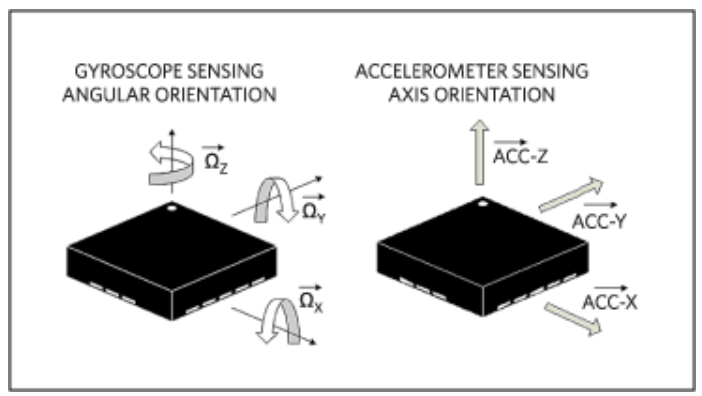
\includegraphics[scale = 0.5]{pictures/IMU/Gyro.png}
    \end{center}
    \caption{Gyroscope and Accelerometer internal axis}
    \label{fig:my_label}
\end{figure}


Each gyroscope channel measures the rate of rotation around one of the internal axes in degrees per second (as our gyroscope has an inbuilt ADC unit, the actual output will be in bits that can be re-interpreted as degrees per second). With these readings, the angular position can be calculated by integrating the gyroscope measurements over time. If the angular velocity is denoted by $\dot{\Theta}$, the angle of rotation can be calculated as follows:

\begin{figure}[H]
    \begin{center}
    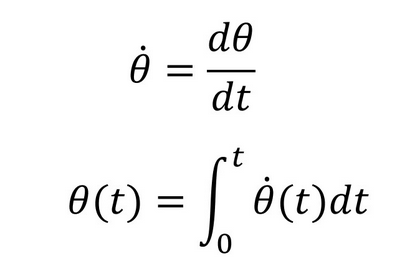
\includegraphics[scale = 0.4]{pictures/IMU/gyro_calculation.png}
    \end{center}
    \caption{Integration of gyroscope readings}
    \label{fig:my_label}
\end{figure}


To better understand the accelerometer readings we can imagine a box with a ball inside of it. In zero gravity conditions the ball would be floating in the air and no force on any of the walls would be detected.


\begin{figure}[H]
    \begin{center}
    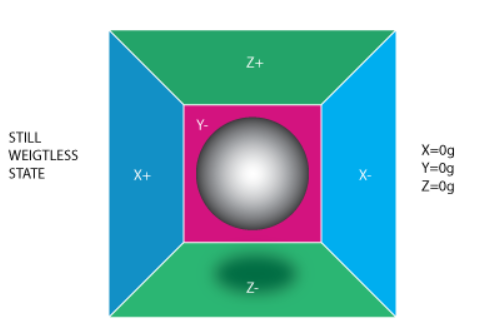
\includegraphics[scale = 0.5]{pictures/IMU/Accel_0grav.png}
    \end{center}
    \caption{Accelerometer, zero gravity and motion on X axis }
    \label{fig:my_label}
\end{figure}

If the box was moved in positive X axis direction with acceleration of $9.81 m/s^2$, the ball would hit the wall of the box in negative X axis direction and register force of $1g$. From this we can note that accelerometer is reading a force in the opposite direction of the motion. 

Similarly we can now imagine that when the box is sitting still in gravitational field of the Earth, we would get a reading of $1g$ in the downwards Z axis direction. If the IMU was rotated in respect to Earth surface, the reading of 1g would be split into x, y and z components on the accelerometer internal axis. We can use these readings to calculate the positional angles with respect to earth surface with the help of the following formula.

\begin{figure}[H]
    \begin{center}
    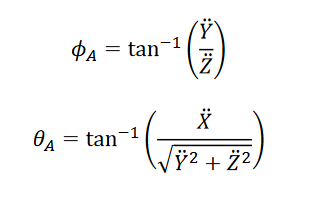
\includegraphics[scale = 0.7]{pictures/IMU/Accel_angles.png}
    \end{center}
    \caption{Positional angle calculation   }
    \label{fig:my_label}
\end{figure}

It is important to note that all measurements on accelorometer are read in the IMU body frame. In order to relate them to Earth's surface we need to choose a reference coordinate system and transform the measurements from the body reference frame to the chosen coordinate system.

For our model we have chosen to work with NED (north-east-down) coordinate system, where X axis is pointing to north, the Y‐axis to east, and the z‐axis is pointing down.

\begin{figure}[H]
    \begin{center}
    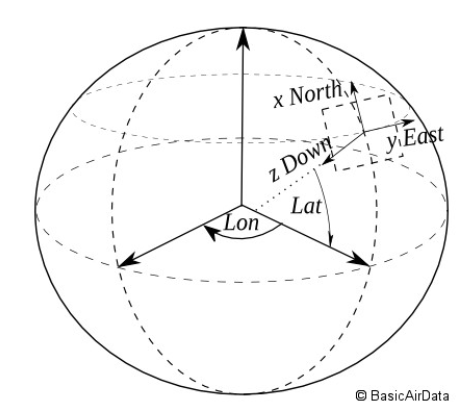
\includegraphics[scale = 0.5]{pictures/IMU/NED_sys.png}
    \end{center}
    \caption{NED coordinate system}
    \label{fig:my_label}
\end{figure}

In order to relate sensor readings from body reference frame to NED, we are using Euler angles, which provide a way to represent the 3D orientation of an object using a combination of three rotations about different axis. Rotation about X axis is denoted by $\Phi$, rotation about Y with $\Theta$ and rotation around Z axis with $\Psi$. 

\begin{figure}[H]
    \begin{center}
    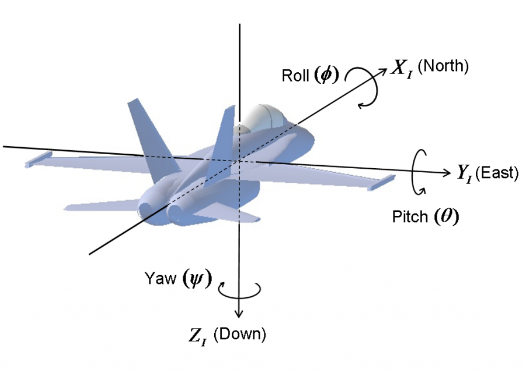
\includegraphics[scale = 0.5]{pictures/IMU/Euler_angles.png}
    \end{center}
    \caption{Euler angles}
    \label{fig:my_label}
\end{figure}

Any object rotation can be described by multiplying a rotational matrix with the original position vector. Any rotation matrix R can be decomposed as a product of three elemental rotation matrices - Roll, Yaw and Pitch.\newline
\begin{figure}[H]
    \begin{center}
    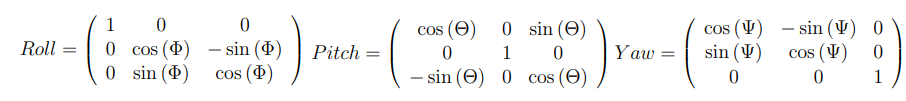
\includegraphics[scale = 0.7]{pictures/IMU/rotational_matrixes.png}
    \end{center}
    \caption{Rotational matrixes}
    \label{fig:my_label}
\end{figure}


The complete rotation matrix for moving from the NED frame to the body frame is achieved by first performing Yaw then Pitch then Roll resulting in the following rotation matrix

$R(\Phi, \Theta, \Psi):$
\newline
\newline
\begin{displaymath}
\resizebox{1.0\textwidth}{!}{
$\left(\begin{array}{ccc}
\cos \left(\Psi \right)\,\cos \left(\Theta \right) & -\cos \left(\Theta \right)\,\sin \left(\Psi \right) & \sin \left(\Theta \right)\\
\cos \left(\Phi \right)\,\sin \left(\Psi \right)+\cos \left(\Psi \right)\,\sin \left(\Phi \right)\,\sin \left(\Theta \right) & \cos \left(\Phi \right)\,\cos \left(\Psi \right)-\sin \left(\Phi \right)\,\sin \left(\Psi \right)\,\sin \left(\Theta \right) & -\cos \left(\Theta \right)\,\sin \left(\Phi \right)\\
\sin \left(\Phi \right)\,\sin \left(\Psi \right)-\cos \left(\Phi \right)\,\cos \left(\Psi \right)\,\sin \left(\Theta \right) & \cos \left(\Psi \right)\,\sin \left(\Phi \right)+\cos \left(\Phi \right)\,\sin \left(\Psi \right)\,\sin \left(\Theta \right) & \cos \left(\Phi \right)\,\cos \left(\Theta \right)
\end{array}\right)$}
\end{displaymath}

To transition from body reference frame to NED, we need to perform the rotations in opposite order - Roll, then Pitch, then Yaw from negative angles
 $R( -\Psi, -\Theta ,-\Phi):$ 

\begin{displaymath}
\resizebox{1.0\textwidth}{!}{
$\left(\begin{array}{ccc}
\cos \left(\Psi \right)\,\cos \left(\Theta \right) & \cos \left(\Phi \right)\,\sin \left(\Psi \right)+\cos \left(\Psi \right)\,\sin \left(\Phi \right)\,\sin \left(\Theta \right) & \sin \left(\Phi \right)\,\sin \left(\Psi \right)-\cos \left(\Phi \right)\,\cos \left(\Psi \right)\,\sin \left(\Theta \right)\\
-\cos \left(\Theta \right)\,\sin \left(\Psi \right) & \cos \left(\Phi \right)\,\cos \left(\Psi \right)-\sin \left(\Phi \right)\,\sin \left(\Psi \right)\,\sin \left(\Theta \right) & \cos \left(\Psi \right)\,\sin \left(\Phi \right)+\cos \left(\Phi \right)\,\sin \left(\Psi \right)\,\sin \left(\Theta \right)\\
\sin \left(\Theta \right) & -\cos \left(\Theta \right)\,\sin \left(\Phi \right) & \cos \left(\Phi \right)\,\cos \left(\Theta \right)
\end{array}\right)$}
\end{displaymath}

\subsection{Sensor fusion}
Now that we have established two methods of obtaining angular position, we must take into account the deficiencies related to each of the methods. The accelerometer has good accuracy when the drone is not accelerating and the only acceleration we are reading is from gravity.
The gyroscope can read quick movements but since the readings are being integrated, any error in the measurements is repeatedly added to the calculated position thereby leading to a drifting signal.

The solution is to introduce either a filter or an observer to fuse the measurements from accelerometer and gyroscope. For our project we have implemented a complimentary filter consisting of a low pass filter on the accelerometer and a high pass filter on gyroscope and summing the filtered signals.
\newline
The transfer functions of low pass and high pass filters in s domain are given below (where $\tau$ is the time constant and $\omega _o$ is the angular cut-off frequency in $rad/s$):\newline 
\begin{displaymath}
H(s) = \frac{V_{out}(s)}{V_{in}(s)} = \frac{\omega_0}{(s+\omega_0)}= \frac{1}{\tau s+1}
\end{displaymath}
\begin{displaymath}
H(s) = \frac{V_{out}(s)}{V_{in}(s)} = \frac{s}{(s+\omega_0)}= \frac{\tau s}{\tau s+1}
\end{displaymath}

Cut-off frequency in Hz:
\begin{displaymath}
    f_c=\frac{\omega _o}{2\pi}
\end{displaymath}
\newline

Since the filter will be digital, the real time transfer function needs to be discretized by moving to the Z domain. This can be done with the help of Bilinear transform (Tustin's method), with the following substitution (where $T_s$ is the sampling time):
\begin{displaymath}
    s=\frac{T_s}{2}\frac{1-z^{-1}}{1+z^{-1}}
\end{displaymath}


 This results in discrete transfer function: 



\begin{displaymath}
    H(z)= \frac{\omega _o}{\frac{T_s}{2}\frac{1-z^{-1}}{1+z^{-1}} + \omega _o}=\frac{b_o + b_1z^{-1}}{1-a_1z^{-1}}
\end{displaymath}

Giving us discrete time implementation of:  
\begin{displaymath}
    y(t)=a_o y_{n-1}+b_ox_n+b_1x_{n-1}
\end{displaymath}

To calculate the coefficients $a_o, b_o, b_1$ we can use Matlab Transfer function $tf()$ and Continuous to discrete time function $c2d() $


\begin{figure}[H]
    \begin{center}
    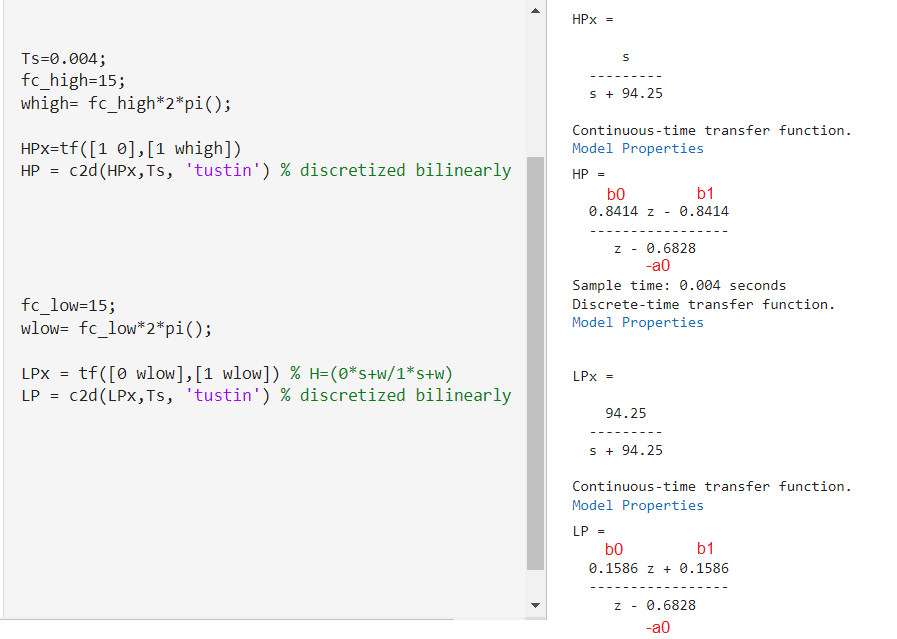
\includegraphics[scale = 0.5]{pictures/IMU/filters_matlab.png}
    \end{center}
    \caption{Bilinear transform in Matlab}
    \label{fig:my_label}
\end{figure}



The sampling time $T_s$ used in calculations is the loop time of the code we run for the drone control.


After the calculated angles are passed through their respective filters, the values can be summed up resulting in a complimentary filter (as shown in the visual below):


\begin{figure}[H]
    \begin{center}
    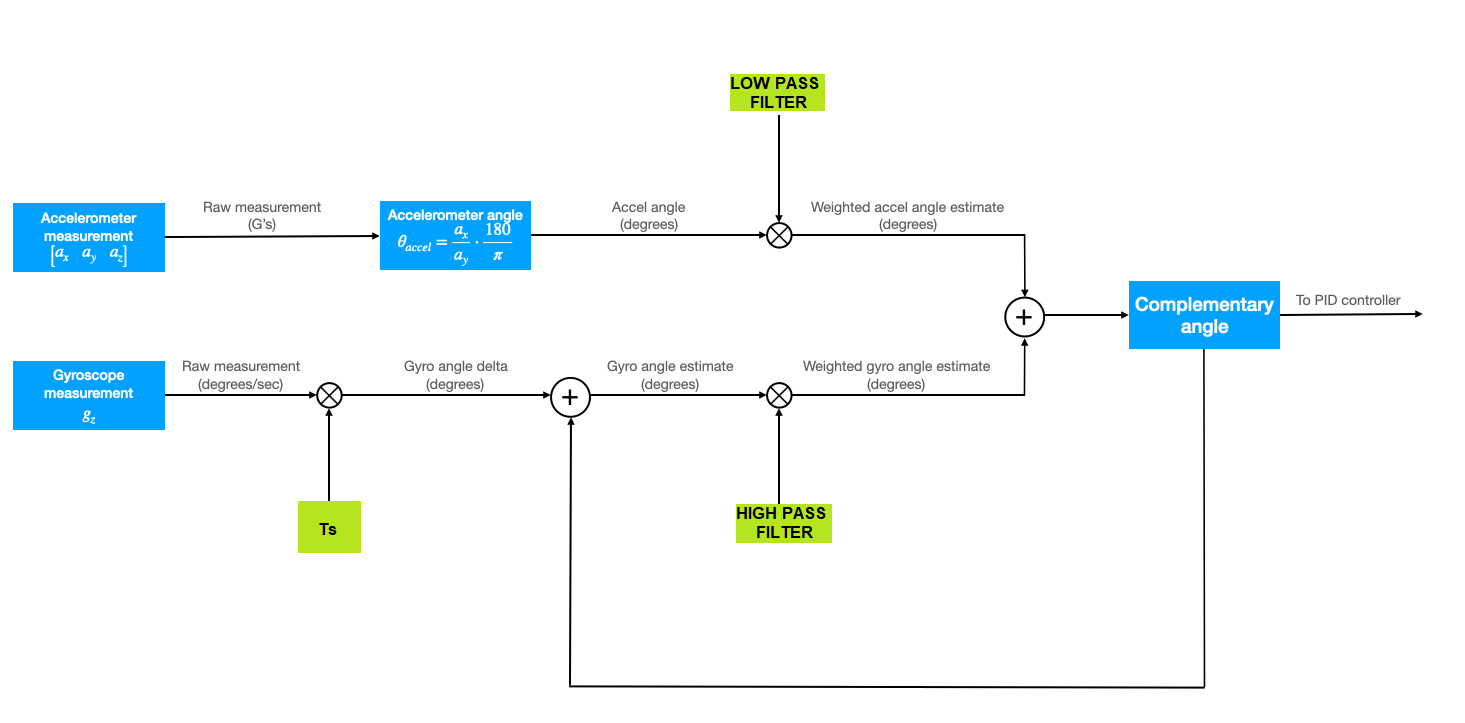
\includegraphics[scale = 0.5]{pictures/IMU/complementary.png}
    \end{center}
    \caption{Complimentary filter implementation in discrete time}
    \label{fig:my_label}
\end{figure}

\subsection{Simulink}

To simulate the IMU readings as feedback in Simulink we first need to consider what input variables will be handled by the gyroscope and the accelerometer plants. The drone plant in the simulation is operating in NED reference frame, therefore any outputs coming from it are also in NED. However the physical IMU sensor will be handling measurements in body reference frame, therefore we need to create a function block to transform the drone output values into body reference frame values. 

For the accelerometer this can be done by taking all linear motion acceleration outputs from drone plant in the form of a column vector $Acc=($X'', Y'', Z''$)$ and multiplying it with the rotational matrix for moving from NED to body. This equation requires knowing the Euler angles to be used in the rotational matrices. These values can also be taken from the drone plant.


\begin{figure}[H]
    \begin{center}
    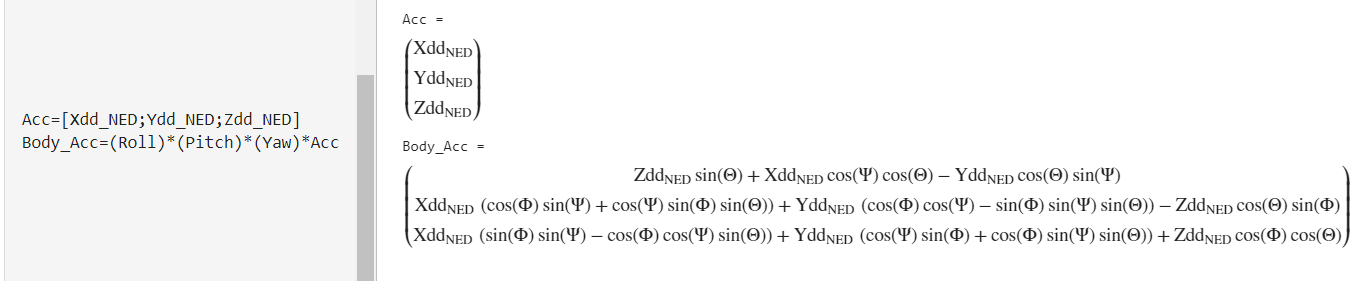
\includegraphics[scale = 0.5]{pictures/IMU/NED_to_body_acc.png}
    \end{center}
    \caption{Rotational transformation from NED to body ref. frame, Matlab}
    \label{fig:my_label}
\end{figure}

\begin{figure}[H]
    \begin{center}
    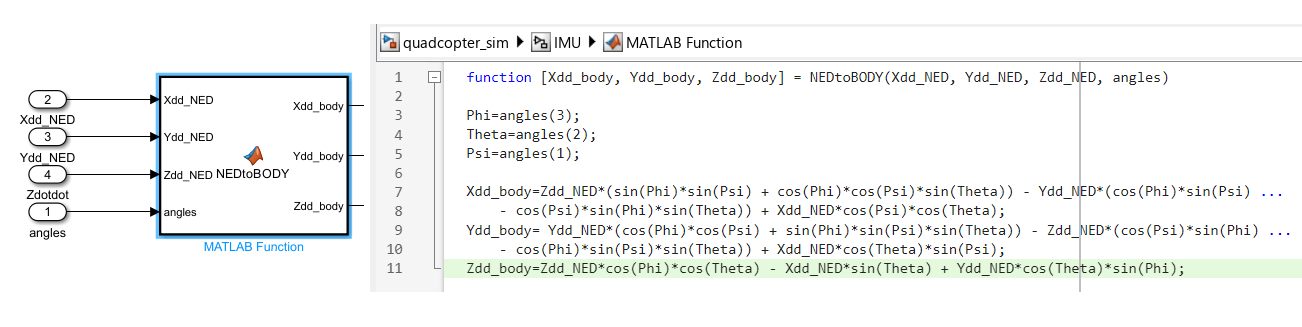
\includegraphics[scale = 0.5]{pictures/IMU/NED_to_bidy_function_block.png}
    \end{center}
    \caption{NED to body transformation function block, Simulink}
    \label{fig:my_label}
\end{figure}

For steady-level flight it can be assumed that angular velocities are the same in body and NED reference frames so we do not need to perform rotational transformation on these values. Therefore the angular velocity output can  be used($\dot{\Phi}, \dot{\Theta}, \dot{\Psi}$,) from the drone plant as the input for the gyroscope plant. 

In the simulation both accelerometer and the gyroscope plants are reading the ideal values from the drone plant, however in the physical model there would be noise present therefore it is needed to generate noise by adding a random number generator on the incoming signals. In the physical IMU there is also a bias on the readings, which can be measured and simulated in the readings.

\begin{figure}[H]
    \begin{center}
    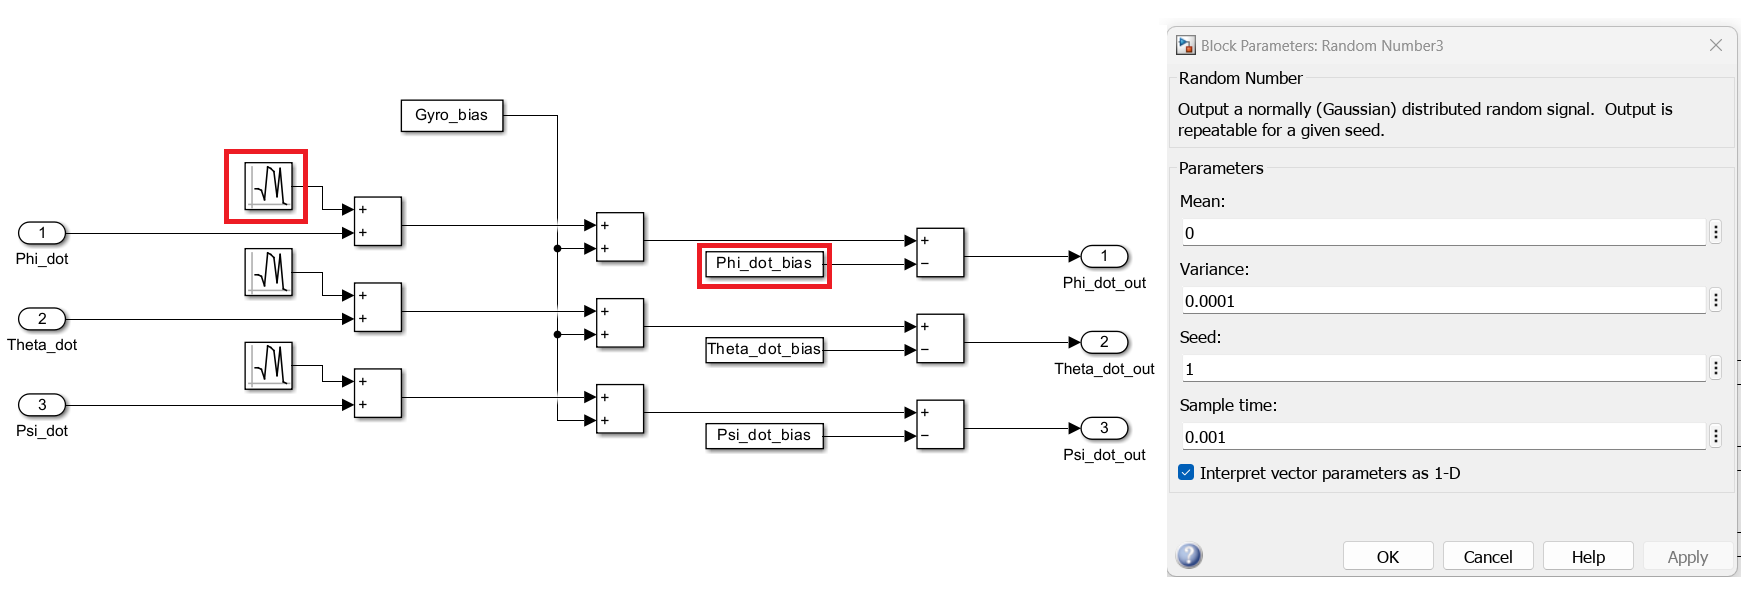
\includegraphics[scale = 0.45]{pictures/IMU/gyro_plant_nr_genrator.png}
    \end{center}
    \caption{Gyroscope plant in Simulink}
    \label{fig:my_label}
\end{figure}

The IMU readings are then passed through the Complimentary filter plant, where gyroscope readings are used to calculate positional angles via integration and passed through a high pass filter and the angles calculated from accelerometer readings are passed through a low pass filter. For the high pass filter the transfer function used is $\frac{T_{high}*s}{T_{high}*s+1}$ where $T_{high}$ is the period of the cutoff frequency of the filter $T_{high}=\frac{1}{f_c}$

\begin{figure}[H]
    \begin{center}
    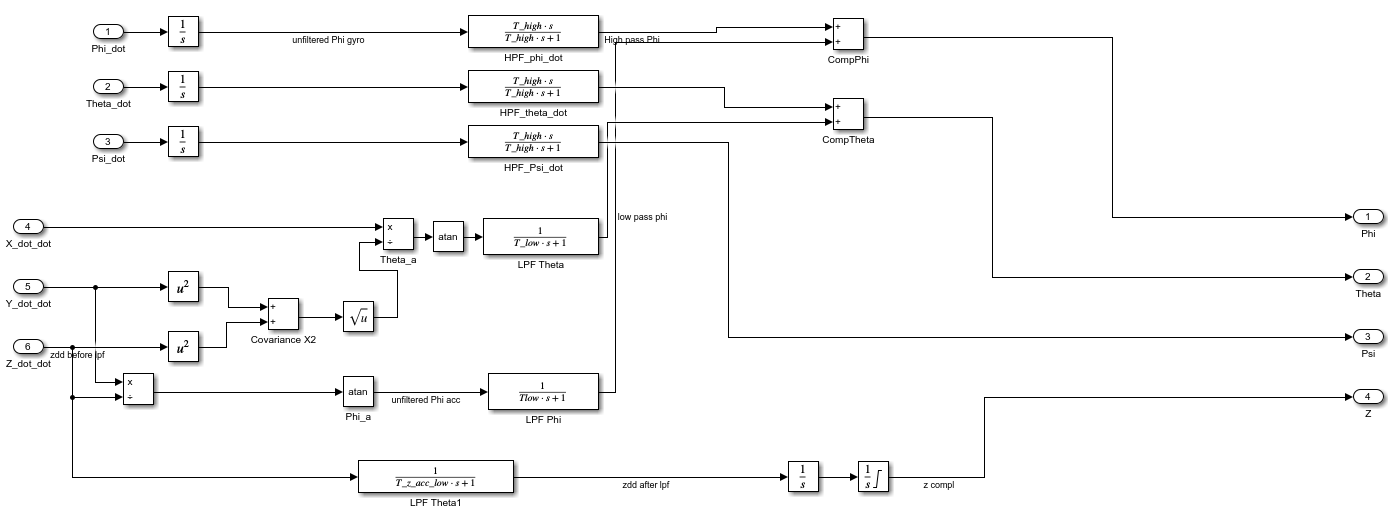
\includegraphics[scale = 0.55]{pictures/IMU/Complimentary_filter_plant.png}
    \end{center}
    \caption{Complimentary filter plant in Simulink}
    \label{fig:my_label}
\end{figure}

The complimentary filter plant also includes calculation of vertical position $Z$ by performing double integration of the vertical acceleration reading. In the physical model the time of flight sensor is included for this measurement, however it is not modeled in the simulation as the sensor was a later addition. In ideal scenario we would also include a sensor that could be used as additional reference for the Yaw, for example, a magnometer, as only using the gyroscope reading to track this angle introduces drift. Unfortunately the drone only has an IMU with 6DOF. 
The filtered values are then converted back to NED reference frame by using calculations described previously and then passed back as feedback input for the control plant.

\begin{figure}[H]
    \begin{center}
    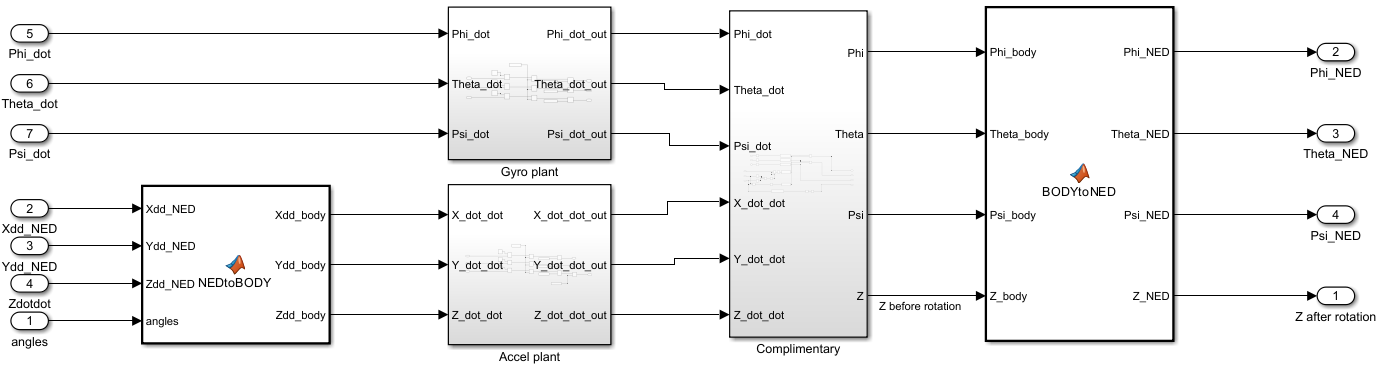
\includegraphics[scale = 0.55]{pictures/IMU/IMU_plant.png}
    \end{center}
    \caption{IMU plant in Simulink}
    \label{fig:my_label}
\end{figure}

\subsection{IMU code}

To obtain the IMU readings from our sensor a connection first needs to be established with the micro-controller board and using Arduino IDE makes this simple by offering Seeed Studio XIAO nRF52840 (Sense) board package. Additionally several libraries need to be included, such as math.h and LSM6DS3.h. 

The LSM6DS3.h pre-defines the I2C address as 0x6B but can be overwritten in code - as in our case the address is 0x6A. 
The library also pre-defines IMU settings - enables both sensors and sets Gyro and Accelerometer sampling rate as 416 Hz. This means sampling time for IMU readings of 2.4 ms, which works with the code for drone control as the sampling frequency is higher than control input calculation frequency. 

By default the maximum range is selected for both sensors - 16g for Accelerometer and 2000 dps for the Gyro. The library also performs the necessary calculations and returns the measurements in gravitational constants and degrees per second and sensor readings can be accessed by using functions readFloatGyroX() and readFloatAccelX().  

\begin{figure}[H]
    \begin{center}
    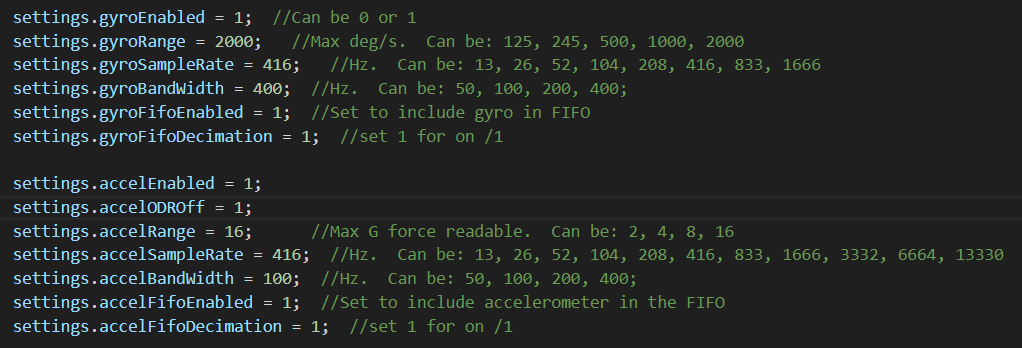
\includegraphics[scale = 0.55]{pictures/IMU/Library_settings.png}
    \end{center}
    \caption{Default settings in LSM6DS3.h library}
    \label{fig:my_label}
\end{figure}


The IMU offers inbuilt analog Low Pass and High pass filters, however it was chosen not to use them and only rely on the digital filters implemented by us.

There are two important additional sensor initiation steps that are not covered by the library - removing sensor bias and aligning the internal axis of the Gyro and Accelerometer units. 

To calibrate the sensor, a simple $for$ loop is used that runs 10 000 iterations reading the sensor output and averages the values. Since we know that when the sensor is sitting still, we should be reading 0 angular velocity, these average readings can be subtracted from every future reading, thus creating the ReadGyro() function. 


\begin{figure}[H]
    \begin{center}
    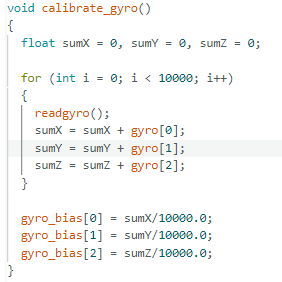
\includegraphics[scale = 0.85]{pictures/IMU/gyro_calibrate.png}
    \end{center}
    \caption{Gyro calibration}
    \label{fig:my_label}
\end{figure}

\begin{figure}[H]
    \begin{center}
    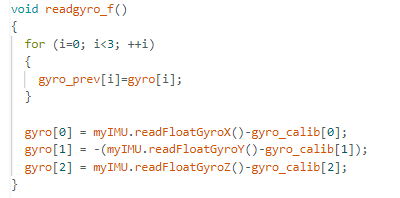
\includegraphics[scale = 0.85]{pictures/IMU/read_gyro_f.png}
    \end{center}
    \caption{$read_gyro_f()$ function}
    \label{fig:my_label}
\end{figure}


To calibrate the accelerometer,  the orientation of the sensor needs to be changed between each $for$ loop to have each of the positive and negative axis pointing downwards. As per instructions in the data sheet the full range of readings on each axis should be 2$g$. 

The second initialization step is to align the axis for gyroscope and accelerometer before using the readings for any further calculations.
The direction of the X,Y,Z axis is pre-set by factory, however it will not be the same for all sensors and since we are using a complimentary filter to fuse the measurements, it is crucial to make sure that the positive direction gyroscope and accelerometer axis are the same and that the positive angle of rotation matches the references used in motor control. \newline
During testing one of the Seeed Xiao micro-controllers was damaged and had to be swapped for a new one. It turned out that on the new micro-controller board the direction of y axis was the opposite for both sensor units and as a result was affecting the filtered sensor readings and the control algorithm. \newline

Several functions needed for our positional calculations is needs to be introduced:
$readGyrof(), readAccf():$\newline
All sensor readings are stored in arrays of 3 float elements - one for each axis reading and since the readings from previous iteration are necessary for the digital filtering, before fetching the new sensor output values, old ones are shifted in a separate array.

$CalcAngleGyroF():$\newline
Calculates the Euler angles by "integrating" the gyroscope readings. It takes the last known angle of attitude and adds the current angular velocity times the time step of the full control loop. This method can be used since the drone will be launched from horizontal position therefore it can be assumed that the inital conditions to be 0.


\begin{figure}[H]
    \begin{center}
    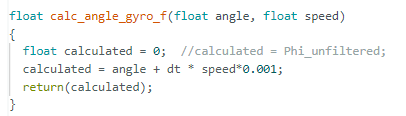
\includegraphics[scale = 0.85]{pictures/IMU/calc_angle_gyro.png}
    \end{center}
    \caption{CalcAngleGyroF() function}
    \label{fig:my_label}
\end{figure}


$UnfiltAngleGyroF(), UnfiltAngleGyroPrevF():$\newline
Needed for the digital filter - calculates unfiltered attitude angles based on current and previous gyroscope readings.

$CalcPhiAccF(), CalcThetaAccF():$\newline
Calculates Phi and Theta from Accelerometer readings interpreting full range of motion to be from $-\Pi$ to $\Pi$.

\begin{figure}[H]
    \begin{center}
    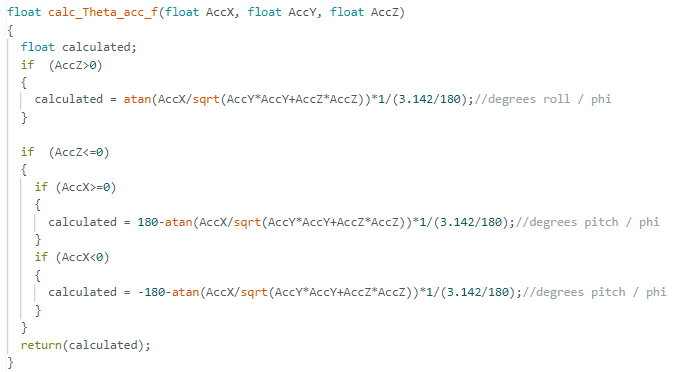
\includegraphics[scale = 0.85]{pictures/IMU/calc_angle_theta.png}
    \end{center}
    \caption{CalcThetaAccF() function}
    \label{fig:my_label}
\end{figure}


$HPFGyroAngleF(), LPFAccAngleF():$\newline

Calculates the values filtered via digital filters. Based on the following discrete time implementation of high pass/ low filters explained earlier in the document:

$y(t)=a_o y_{n-1}+b_ox_n+b_1x_{n-1}  $


A function can be created to carry out this calculation, where $y_{n-1}$ is the previous filtered value, $x_n$ is the unfiltered value based on current readings and $x_{n-1}$ is the unfiltered value based on previous readings. The structure of both high pass and low pass filters is the same, however the coefficients calculated by the Bilinear transform differ. Most notably - the 
$b1$ coefficient for High pass filter is negative.

\begin{figure}[H]
    \begin{center}
    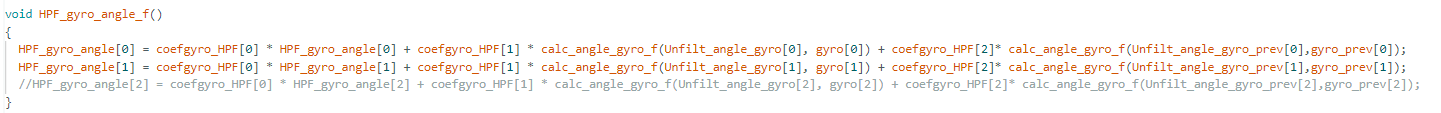
\includegraphics[scale = 0.85]{pictures/IMU/HPF_gyro.png}
    \end{center}
    \caption{HPFGyroAngleF() function}
    \label{fig:my_label}
\end{figure}

\begin{figure}[H]
    \begin{center}
    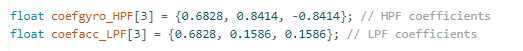
\includegraphics[scale = 0.85]{pictures/IMU/HPF_LPF_coefff.png}
    \end{center}
    \caption{Digital filter Bilinear transform coefficients}
    \label{fig:my_label}
\end{figure}


$ComplimentaryF()$
\newline

Combines high pass and low pass filter output.
For the time of flight sensor it is needed to include the $Adafruit_VL53L0X.h$ library which then allows the vertical distance to be measured with the help of measure.RangeMilliMeter function.
However it is needed to remember that the drone could be pitched and rolled therefor to get an accurate hight, we need to triangulate the reading based on the Roll and Pitch angles.
This can be done with the help of rotational matrix as follows:


\begin{figure}[H]
    \begin{center}
    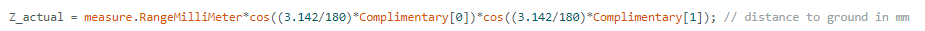
\includegraphics[scale = 0.85]{pictures/IMU/Z_actual_trinagulation.png}
    \end{center}
    \caption{Calculating Z position from time of flight sensor}
    \label{fig:my_label}
\end{figure}



To choose optimal cut-off frequencies for the digital filters, the Complimentary filter output can be printed alongside the unfiltered Euler angles from gyroscope and accelerometer to see how much the filtered signal is attenuated and observe the phase shift. 


\begin{figure}[H]
    \begin{center}
    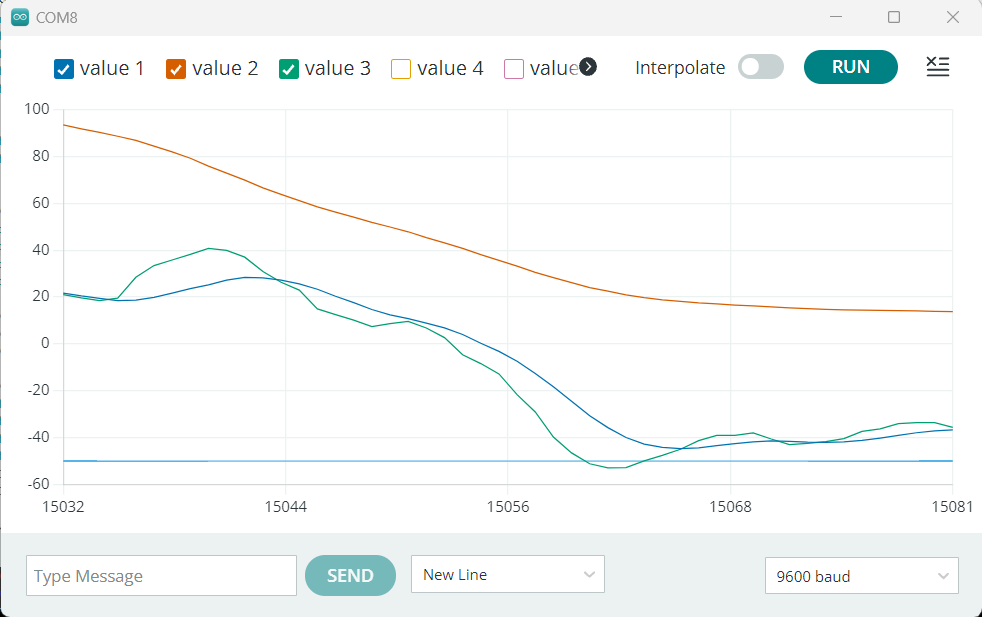
\includegraphics[scale = 0.65]{pictures/IMU/M5.png}
    \end{center}
    \caption{Complimentary filter output vs unfiltered values}
    \label{fig:my_label}
\end{figure}
